\cotefile{126}
\scanpage{19}
% @ upper left, printed letterhead
% letterhead
M. DUFOUR\\
VARITYPISTE\\
131, \textsc{Rue Lecourbe}\\
PARIS XV\textsuperscript{e}\\
$\blacksquare$\\
C. C. P. Paris 14.143-34\\
R. M. 140.029

% @ 1–2, top right
% Four oblique cancellation strokes traverse the manuscript draft.
\deleted{Soit $I=[1,\ldots,\unsure{n}]$. Considérons}
\[
\deleted{Y'=\operatorname{Hom}(I,X)=X^I}
\]

% @ 3–5, upper half
\deleted{On a donc un $Y$-morphisme naturel}
\[
\deleted{Y'\times I\longrightarrow X}
\]
\deleted{i.e. un $Y'$-morphisme naturel}
\[
\deleted{f:\deleted{\unsure{X|Y}}Y'\times I\longrightarrow X'}
\]

% @ 6–8, across fold
\deleted{[correspondant aux $n$ projections $\operatorname{pr}_{\unsure{\alpha|i}}:Y'=X^I\to X$]}

\deleted{Pour tout $y'\in Y'$, on en conclut un \unsure{hom|morphisme}}
\[
\deleted{I\times\operatorname{Spec}\deleted{\unsure{K}}k(y')\longrightarrow X'\times_{\unsure{Y|Y'}}\operatorname{Spec}k(y')}
\]

% @ 9–12, middle and lower right
\deleted{\uline{Lemme} L'\unsure{ens|ensemble} \inserted{$Y''$} des pts de $Y'$ où le morphisme précédent est bijectif est à la fois ouvert et fermé, et \deleted{il s'applique} \inserted{$Y''\to Y$} \deleted{bijectivement} surjectif\deleted{\unsure{ement sur $Y$}}.}

% @ 13–17, bottom and left margin
% slanted
\deleted{\inserted{$Y''$ est aussi} L'ens des pts où $I\times\operatorname{Spec}k(y')\to X'_{y'}$ \deleted{est} \inserted{\unsure{doit être explicité|doit être considéré|décrit des conditions} \unsure{ds|dans|de 2} le \unsure{lemme|lemmes}} \uline{géométriquement} \uline{injectif}, ou encore où c'est \uline{radiciel}, ou encore où c'est un \uline{monomorphisme} [= imm. fermée]}

% @ 18, bottom edge
\deleted{On sait (\deleted{\unsure{déjà|décrit}}\inserted{$Y'\times I$ est plat propre sur $Y'$}) que c'est un ouvert.}
% @ central sideways watermark
% printed form
\textsc{Extra Strong}\\
\unsure{Guerimand|Guérimand} Voiron
% archive sheet number: 18

\scanpage{20}
% @ upper left, letterhead
% letterhead
M. DUFOUR\\
VARITYPISTE\\
131, \textsc{Rue Lecourbe}\\
PARIS XV\textsuperscript{e}\\
$\blacksquare$\\
C. C. P. Paris 14.143-34\\
R. M. 140.029

% @ 1–3, at the head and right of the letterhead
\uline{Lemme} \unsure{!}
Si $X\xrightarrow{f}Y$ admet une section \deleted{\unsure{$s$}}$s$, alors $s(Y)$ est à la fois \deleted{\unsure{ouvert}} \uline{fermé} et \uuline{ouvert}. En effet,

% @ left margin, beside 4–6
\margin{\figure{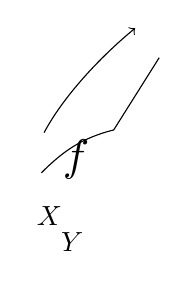
\begin{tikzpicture}[x=.34cm,y=.34cm]
\draw[thin,->] (.2,3.0) .. controls (1,4.5) and (2.5,6.0) .. (3.6,6.9);
\draw[thin] (.1,1.5) .. controls (.9,2.3) and (1.6,2.8) .. (2.8,3.1) -- (4.5,5.8);
\node[scale=1.6] at (1.4,2.0) {$\unsure{f}$};
\node at (.4,-.1) {$X$}; \node at (1.25,-1.1) {$Y$};
\end{tikzpicture}}}

% @ 4–11, heavily cancelled central argument
\deleted{on voit de suite que c'est une réunion $X'$ de composantes irréductibles de $X$ [$X\to Y$ est fini] il faut montrer que si \deleted{\unsure{une}} $X''$ est \deleted{une} la réunion des autres composantes irréductibles, alors $X'\cap X''=\varnothing$. Or \deleted{\unsure{on a que}} \unsure{générique de|qu'en un pt de|l'image} \unsure{une|un} composante de $Y$, on \unsure{$\nu''(y)=n-1$|$d''(y)=n-1$}, donc les composantes irréductibles de}

% @ 12–16, under the cancelled argument
Pour ce dernier point on est ramené au cas où $Y$ est irréductible [car si les $Y_i$ sont les composantes de $Y$, il suffit de prouver que $s(\unsure{y|Y|Y_i})$ induit un ouvert sur chaque $f^{-1}(\unsure{Y|Y_i})$], or alors les composantes irréductibles de $X$ sont \uline{disjointes} [\unsure{vif|vérif}], \unsure{en} \deleted{\unsure{par exemple}} d'où la conclusion.

% @ left margin, level with the reduction to components
\margin{\diagram{\begin{tikzcd}[ampersand replacement=\&,column sep=tiny,row sep=small]
X\arrow[d]\&\deleted{\unsure{=X}}\displaystyle\bigcup_i f^{-1}(Y_i)\arrow[d] \\
Y\arrow[u,bend left=35,"s"]\&{}=\displaystyle\bigcup_i Y_i\arrow[u,bend left=35,"s_i"]
\end{tikzcd}}}

% @ 17–18, foot
Donc on aura $X=X_{(1)}\amalg X^{(1)}$, où $\unsure{\nu|v|d}(X_{(1)}/Y)=1$, $\nu(X^{(1)}/Y)=n-1$.
% @ central sideways watermark
% printed form
\textsc{Extra Strong}\\
\unsure{Guerimand|Guérimand} Voiron
% archive sheet number: 19

\scanpage{21}
% @ 1–4, upper third
et que $y'\in Y''\iff$ il existe un voisinage $U$ de $y'$ \unsure{ds|de|dans} $Y'$ tel que $f\ U\times I\to X'|U$ soit une \deleted{\unsure{imm.}} imm. fermée. Le complémentaire de $Y''$ est formé des pts tels que

% @ 5–6, upper third
\[
I\times\operatorname{Spec}k(y')\longrightarrow X'\times_Y\operatorname{Spec}k(y)
\]
soit \unsure{géométriquemt|géométriquement} non injectif,
% @ centre and upper right, paper and show-through
% printed form
\textsc{Extra Strong}\\
\unsure{Guerimand|Guérimand} Voiron
% Upper right: M. DUFOUR letterhead showing through from the reverse.
% archive sheet number: 20

\scanpage{22}
% @ 1–3, top
Faisant des extensions de la base successives $Y_1=X$, [d'où $X_1^{\deleted{\unsure{*}}}=X\times_Y Y_1$, $X_1=X_{(1)}\amalg X^{(1)}$, puis $Y_2=X^{(1)}$,] on trouve

% @ 4–9, bracketed lemma
\uline{Lemme} 2 Il existe un $Y'\deleted{_{\unsure{2}}}$ \deleted{\unsure{sur}} fini sur $Y$, avec $Y'\deleted{_{\unsure{2}}}\to Y$ surjectif [et \deleted{radiciel} \inserted{univ\textsuperscript{t} ouvert} si on veut] tel que $X'=X\times_Y Y'$ se décompose en $n$ \unsure{variétés|revêtements|réunion} $X'_i$ connexes de degré \deleted{fini} séparable $1$ sur $Y$.

% @ 10–16, below the fold
Soit $I$ l'ens des composantes connexes de $X'$, \unsure{considérons|considérer} $Y'\times I$ comme rev. étale de $Y'$. Il est trivial que $X'_0=Y'\times I$ est muni d'une donnée de descente \unsure{relat\textsuperscript{vt} à|relativement à} $Y'\to Y$, d'où un \uline{rev.} \uline{étale} $X$ de $Y$, donnant $X'_0{}^{\deleted{\unsure{*}}}$ par image inverse.

% @ lower left, level with 15–18
\margin{\diagram{\begin{tikzcd}[ampersand replacement=\&,row sep=small,column sep=small]
X_{0}^{\deleted{\unsure{*}}}\arrow[d]\&\&X'_{0}{}^{\deleted{\unsure{*}}}\arrow[ll]\arrow[d]\\
Y\&\&Y'\arrow[ll]\\
\&Y^{*}_{\deleted{\unsure{2}}}\arrow[ul]\&\&Y'{}^{*}_{\deleted{\unsure{2}}}\arrow[ul]\arrow[ll]
\end{tikzcd}}}

% @ 17–19, foot
Soit ${\unsure{Y|Y'}}^{*}_{\deleted{\unsure{2}}}$ un rev. \uline{étale} [donc plat] de $Y$ qui décompose $X_0$ complètement, prenons l'image inverse de la situation sur
% @ sideways band through the manuscript
% printed form
\textsc{Extra Strong}\\
\unsure{Guerimand|Guérimand} Voiron
% archive sheet number: 21

\scanpage{23}
% @ upper left, letterhead
% letterhead
M. DUFOUR\\
VARITYPISTE\\
131, \textsc{Rue Lecourbe}\\
PARIS XV\textsuperscript{e}\\
$\blacksquare$\\
C. C. P. Paris 14.143-34\\
R. M. 140.029

% @ 1–4, top
$Y^{*}_{\deleted{\unsure{1}}}$, Donc maintenant on est dans le cas où la descente de $X'{}^{*}$ donne un $Y'{}^{*}$ complètement décomposé\deleted{\unsure{s}}.

% @ 5–10, above fold
Il en résulte aisément que les composantes connexes de $X'{}^{*}$ sont les images inverses des composantes connexes de $X^{*}$ (\uline{\unsure{noter|cf.} Lemme} 3] compte tenu que \deleted{$\unsure{X\to|X\leftarrow|X}$} $Y'{}^{*}\to Y^{*}$ est univ.\textsuperscript{t} ouvert. Donc

% @ 11–14, bracketed lemma
\uline{Lemme 4} Il existe un rev. étale surjectif $Y^{*}\longrightarrow Y$ tel que $X^{*}=X\times_Y Y^{*}$ ait des composantes connexes qui sont de degré $1$ sur $Y^{*}$.

% @ 15–19, bottom
Le morphisme canonique
\[
X^{*}\longrightarrow Y^{*}\times I=X^{*}_0
\]
[$I$ ens des composantes connexes de $X^{*}$] est compatible \deleted{\unsure{trivialemt}} \inserted{par définition} avec les \unsure{structures|données} de descente sur $Y^{*}\times I$, (et $X^{*}$), \unsure{\textbackslash}
% @ sideways watermark through the text
% printed form
\textsc{Extra Strong}\\
\unsure{Guerimand|Guérimand} Voiron
% archive sheet number: 22

\scanpage{24}
% @ 1–3, top
donc définit un morphisme \deleted{canonique}
\[
X\longrightarrow X_0
\]
qui est surjectif radiciel fini.

% @ 3–12, middle
Pour montrer que ce morphisme est bien solution du \unsure{Pb} universel que nous avions dit, on voit que sur $Y^{*}$, un morphisme de $X^{*}$ dans un \unsure{revêtt|revêtement} étale $Y'{}^{*}$ de $Y^{*}$ se factorise de façon unique en
\[
X^{*}\unsure{-|\to} X_0^{*}\longrightarrow Y'{}^{*}
\]
[et si $Y'{}^{*}$ provient d'un $Y'$, alors le morphisme donné est compatible avec les données de descente \deleted{\unsure{ssi}} $X^{*}_0\to Y'{}^{*}$ l'est] Pour vérifier ce fait, on est ramené aussitôt au cas où $X^{*}_0=Y^{*}$, où c'est immédiat \unsure{---} (\unsure{vu -- lemme|ou -- lemme|cf. lemme}).

% @ 16–19, lower paragraph
\uline{À \deleted{\unsure{vérifier}}} \uline{généraliser} au cas où on a un morphisme \unsure{propre} \uline{univ\textsuperscript{t} ouvert} $X\to Y$ dans lequel les composantes connexes \inserted{absolues} des fibres ``se comportent bien'' i.e. en nb \inserted{loc} constant \deleted{\unsure{et}}

% @ 20–21, foot
\uline{Question} Caractérisation des foncteurs représentables par des rev. étales ???
% @ middle, watermark and reverse letterhead
% printed form
\textsc{Extra Strong}\\
\unsure{Guerimand|Guérimand} Voiron
% The reversed letterhead at upper right shows through from the other face.
% archive sheet number: 23

\scanpage{25}
% @ upper left, letterhead
% letterhead
M. DUFOUR\\
VARITYPISTE\\
131, \textsc{Rue Lecourbe}\\
PARIS XV\textsuperscript{e}\\
$\blacksquare$\\
C. C. P. Paris 14.143-34\\
R. M. 140.029

% @ central watermark, turned 90 degrees
% printed form
\textsc{Extra Strong}\\
\unsure{Guerimand|Guérimand} Voiron
% archive sheet number: 24

\scanpage{27}
% @ 1–3, top
$S$ schéma noethérien

$T/S$ de type fini, \deleted{\unsure{fid.}} plat

$U$ partie ouverte dense de $T\times_S T$, $V$ partie ouverte dense de $T\times_S T\times_S T$, $V\subset\deleted{\unsure{p}}\bigcap_{i\ne j}p_{ij}^{(3)-1}(U)$

% @ 4–5, top, revision on second line
$F$ catégorie fibrée sur la catégorie des $S$-schémas de type fini, on suppose \deleted{\unsure{$F/S$|$F_S$}} \unsure{ses|les} \deleted{\unsure{morphismes}} \inserted{\unsure{ses}} morphismes \deleted{\unsure{de $F$|fid. plats}} \inserted{\unsure{d'objets sont des morphismes de|$S$-schémas de type fini}} $F$-descente \deleted{\unsure{universelle}}

$X\in F_S$

% @ 6, cocycle equation
\[
\varphi:(X\times_S T)|\unsure{U|\mathcal{U}}\xrightarrow{\sim}(T\times_S X)|U
\]
On suppose $p_{13}^{*}(\varphi)={p}_{23}^{*}(\varphi)\,p_{12}^{*}(\varphi)$ au dessus de $V$

% @ 7–10, proposition
\uline{Proposition} Sous ces conditions il existe une partie ouverte dense $T'$ \deleted{$U'$ $\subset U$ de $T\times_S T$ telle que $\varphi|U'$ soit} de $T$, et une \uline{donnée de descente} $\varphi':X\times_S T'\xrightarrow{\sim}T'\times_S X$ telles que $\varphi=\varphi'$ \deleted{\unsure{au}} dessus de. $U\cap(T'\times_S T')=U'$

% @ 11–17, symmetry and density
On peut supposer $U,V$ \uline{invariants par les groupes symétriques}

Il existe une partie \inserted{ouverte} dense $U_{1}{}^{\deleted{\unsure{\prime}}}$ de $U$ telle que $\tau\in U_1\Rightarrow V\cap p_{ij}^{(3)-1}(\tau)$ dense dans $p_{ij}^{-1}(\tau)$ pour tout couple $(i,j)$ avec $i\ne j$ [cf. un lemme qui vient plus bas]. Remplaçant $U$ par $U_1$, on peut donc supposer que \uline{$\tau\in U\Rightarrow V\cap p_{ij}^{(3)-1}(\tau)$ dense \deleted{dans} $p_{ij}^{(3)-1}(\tau)$ pour} $(i,j)$ \uline{tel que} $i\ne j$. \unsure{De même|De m\textsuperscript{e}}, on peut trouver une partie ouverte $T'_{\deleted{\unsure{1}}}$ de $T$ telle que $t\in T'\Rightarrow p_i^{-1}(t)\cap U$ est dense dans $p_i^{-1}(t)$ pour $i=1,2$.

% @ 18–20, reduction and cancellation
Remplaçant $T$ par $T'$ (ce qui est loisible) on peut supposer que \uline{$t\in T\Rightarrow U\cap p_i^{-1}(t)$ dense dans $V$ pour $i=1,2$}

\deleted{Enfin, pour la commodité, on \unsure{Enfin, on suppose|Enfin, on supposera} \uuline{$U$ symétrique}}

% @ 21–25, foot
On désigne par $\xi$ un schéma de type fini variable sur $S$ [pour \unsure{prendre|parler} les pts à valeurs dans $\xi$]. On posera
\[
W=p_{12}^{(3)-1}(U)\cap p_{\unsure{22|23}}^{(3)-1}(U)
\]
et on considère
\[
\pi:W\longrightarrow T\times T\qquad\text{induit par }p_{13}
\]
% archive sheet number: 26

\scanpage{28}
% @ 1–5, top
On considère $X_i=p_i^{*}(X)$ $(i=1,2)$, on va définir un isomorphisme
\[
\deleted{\unsure{\varphi}}\ \psi:\pi^{*}(X_1)\simeq\pi^{*}(X_2)
\]
compatible avec la projection $\pi:W\longrightarrow T\times_S T$, i.e. dont les images inverses sur $W\times_{\pi}W$ \unsure{soient|sont} les \unsure{\^{m}s|m\textsuperscript{es}|mêmes}.

% @ 6–8, cancelled box
\deleted{Pour ceci, on note que}
\[
\begin{aligned}
&\deleted{\pi^{*}(X_1)\simeq p_{\unsure{12|22}}^{(3)*}(X\times_S T|U)}\\
&\deleted{\pi^{*}(X_2)\simeq p_{23}^{(3)*}(T\times_S X|U)}
\end{aligned}
\]

% @ 9–12, middle
Pour ceci, on considère les $\deleted{\unsure{p}}q_i^{(3)*}(X)$ $(i=1,2,3)$,
% slanted
\margin{les $q_i$ induits sur $W$ par les $p_i^{(3)}$}
on note que $\deleted{\unsure{p}}q_1^{(3)*}(X)=\pi^{*}(X_1)$, $\deleted{\unsure{p}}q_3^{(3)*}(X)\simeq\pi^{*}(X_2)$, et qu'on peut considérer le composé
\[
\deleted{\unsure{p}}q_1^{\deleted{\unsure{(3)}}*}(X)\xrightarrow{\sim}\deleted{\unsure{p}}q_2^{\deleted{\unsure{(3)}}*}(X)\xrightarrow{\sim}q_3^{*}(X)
\]

% @ 13–16, lower middle and left margin
Pour prouver la compatibilité de $\psi$ avec $\pi$,
% slanted
\margin{\uline{Question} \uline{de rédaction}}
\deleted{on \unsure{voit|vérifie} $W$}
on écrit $W\times_{T\times_S T}W\subset$
\diagram{\begin{tikzcd}[ampersand replacement=\&,column sep=tiny,row sep=tiny]
T\arrow[d]\&{}\times_S T\arrow[d]\&{}\times_S T\arrow[d]\&{}\times_S T\arrow[d]\\
t_1,\&t',\&t'',\&t_2
\end{tikzcd}}
, et on considère le \deleted{produit} \inserted{sous-objet \deleted{\unsure{ouvert}} $W'$} de
\diagram{\(\begin{array}{ccccccccc}T&\times_S&T&\times_S&T&\times_S&T&\times_S&T\\t_1&&t'&&t''&&t_2&&t'''\end{array}\)}
\deleted{\unsure{formé des septi}} \deleted{\unsure{formé}} correspondant aux \unsure{systèmes|septèmes} $(t_1,t',t'',t_2,t''')$ tels que \deleted{$(t''',t_1),(t''',t_2),(t''',t')$ soient dans $U(\xi)$}
\inserted{$(t''',\deleted{\unsure{t_2}}t',t_1^{\deleted{\unsure{4}}}),(t''',t',t_2)$, \deleted{$(t''',t'')$} $(t''',t'',t_1),(t''',t'',t_2),(t''',t_1,t_2)\in V$.}

% @ lower left, diagram
\diagram{\begin{tikzcd}[ampersand replacement=\&,column sep=small,row sep=small]
\&t'\arrow[dr,"U"]\&\\
t_1\arrow[ur,"U"]\arrow[r,"U"]\arrow[dr,"U"']\&t'''\arrow[u,"U"']\arrow[d,"U"]\arrow[r,"U"]\&t_2\\
\&t''\arrow[ur,"U"']\&
\end{tikzcd}}

% @ final two lines and cancelled formula
On aura donc, si $t_1,t',t'',t_2,t'''$ sont comme il a été spécifié,
\[
\deleted{\varphi_{t_2t'}\varphi_{t't_{2}}=(\varphi_{t_2t'''}\varphi_{t'''t'})(\varphi}
\]
% archive sheet number: 27

\scanpage{29}
% @ 1–5, three identities at the top
\[
\varphi_{t_2t'}\varphi_{t't_1}=\varphi_{t_2\unsure{t'|t_1}}(\varphi_{t't'''}\varphi_{t'''t_1})=(\varphi_{t_2t'}\varphi_{t't'''})\varphi_{\unsure{t''|t'''}t_1}=\varphi_{t_2\unsure{t''|t'''}}\varphi_{t'''t_1}
\]
On voit de \unsure{m\textsuperscript{e}|même} que l'on aura
\[
\varphi_{t_2t''}\varphi_{t'',t_1}=\varphi_{t_2t'''}\varphi_{t'''t_1}
\]
d'où \unsure{par comparaison|en comparant|la compatibilité}
\[
\varphi_{t_2t'}\varphi_{t't_1}=\varphi_{t_2t''}\varphi_{t'',t_1}
\]

% @ 6–10, above fold
Or nous verrons (lemme) que \uline{$W'\to$ \deleted{\unsure{$W\times W$}} \inserted{$W\times_{T\times_S T}W\simeqT^4$ est} surjectif}

Il s'ensuit, comme il est plat, que c'est un morphisme de $F$-descente, donc que $\psi$ est bien compatible avec la projection $\pi:W\to T\times_S T$,

% @ 10–15, at fold
On verra de \unsure{m\textsuperscript{e}|même} (lemme) que \uline{$W\to T\times_S T$ est surjectif}, donc, comme il est plat, il s'ensuit que c'est un morphisme de $F$-descente, donc $\psi$ provient d'un isom.
\[
\varphi':X_1\xrightarrow{\sim}X_2
\]

% @ 16–20, lower right
Montrons que c'est une \deleted{\unsure{Donn}} \inserted{donnée} de descente, donc
\[
\varphi'_{t_3t_2}\varphi'_{t_2t_1}=\varphi'_{t_3t_1}\quad (\text{sur }T\times_S T\times_S T].
\]
Pour ceci, on regarde le \deleted{partie} sous-objet \deleted{\unsure{$W$|$W''$}} \inserted{$W'''$} de $T^6$ formé des $t_1,t_2,t_3,t',t'',t'''$ tels que
\[
(t_1,t'),(t',t_2),(t_2,t'''),(t''',t_3)\in U,\quad\text{et }(t_1,t',t'''),(t''',t'',t_3)\in V
\]

% @ lower left, beside the descent relation
\margin{\diagram{\begin{tikzcd}[ampersand replacement=\&,column sep=tiny,row sep=tiny]
\&\&t'''\arrow[dr,dash]\arrow[ddrr,bend left=38,"U"]\&\&\\
\&t'\arrow[ur]\arrow[dr]\&\&t''\arrow[dr]\&\\
t_1\arrow[ur]\arrow[uurr,bend left=38,"U"]\&\&t_2\arrow[ur]\&\&t_3
\end{tikzcd}}}

% @ 21–22, bottom
On a $W''\to T\times_S T\times_S T$, on va prouver la relation \deleted{\unsure{déduite}} de celle à démontrer par pull-back.
% archive sheet number: 28

\scanpage{30}
% @ 1–5, upper calculation
Par définition, le premier \unsure{mb|membre} devient
\[
(\varphi_{t_3t''}\varphi_{t''t_2})(\varphi_{t_2t'}\varphi_{t't_1})\tag*{\unsure{$\alpha_1$|$\alpha)$}}
\]
Or on a
\[
\varphi_{t''t_2}\varphi_{t_2t'}=\varphi_{t''t'''}\varphi_{t'''t'}\quad [=\varphi'_{t''t'}]
\]
donc la \deleted{\unsure{première}} expression $\unsure{\alpha_1}$ est égale à
\[
(\varphi_{t_3t''}\varphi_{t''t'''})
(\varphi_{t'''t'}\varphi_{t',t_1})\deleted{\unsure{=}}
\]

% @ 6–8, above central space
La première parenthèse, parce que $(t''',t'',t_3)\in V$, est égale à $\varphi_{t_3t'''}$, de \unsure{m\textsuperscript{e}} la deuxième est égale à $\varphi_{t'''t_1}$ ; donc le composé est $\varphi'_{t_3t_1}$ par définition.

% @ 9–13, around the fold
Enfin, prouvons que \deleted{\unsure{sur}} dessus de $U$, $\varphi$ et $\varphi'$ \unsure{coïncident} : on \deleted{\unsure{est ramené à prouver que|on est ramené}} \inserted{note pour ceci que} $V\xrightarrow{p_{13}}U$ est surjectif, \deleted{\unsure{donc}} donc on est ramené à prouver l'assertion \unsure{analogue|sur la figure} en se \unsure{remontant|ramenant} sur \unsure{$V$|$U$}, laquelle est triviale.

% @ middle left, three points beside projection
\margin{\diagram{\begin{tikzcd}[ampersand replacement=\&,column sep=tiny,row sep=tiny]
\&\deleted{\unsure{t_3}}t'\arrow[dr,dash]\&\\
t_1\arrow[ur,dash]\&\&t_2
\end{tikzcd}}}

% @ 14, separate line
La démonstration des lemmes est facile

% @ 15–20, foot
\uline{Corollaire à la proposition} Supposons que pour toute partie ouverte dense $T'$ de $T$, d'image $S'$ (ouverte) dans $S$, $T'\to S'$ soit un morphisme de $F$-descente \uline{stricte}. Alors on peut trouver \inserted{un ouvert dense $T'$ de $T$, et un} $Y\in F_{S'}\deleted{\unsure{\xi}}$, \deleted{\unsure{tel que}} un isom $X\simeq Y\times_{S'}T'$, compatible avec \unsure{la donnée|les données} de descente
% archive sheet number: 29

\scanpage{32}
% @ 1–6, top
Question de la possibilité de descente par un morphisme fid. plat \uline{non fini}. Un cas type est le suivant : Soit $T$ \deleted{\unsure{plat et|plat}} \inserted{étalé gal.} fini sur $S$, de groupe $G$, et \deleted{\unsure{enlevons}} soit $T'$ l'ouvert \deleted{$T-\unsure{f^{-1}(s)}$ de $T$, \unsure{où} $\unsure{s}$} $T-D$, où $D=f^{-1}(s)-(t)$ $(f(t)=s)$, --- $s$ étant un pt fermé de $S$. \inserted{On suppose \unsure{qu'il|que} \deleted{\unsure{y a}} $f^{-1}(s)$ a $n$ pts}.

% @ upper left, preliminary diagram
\margin{\diagram{\begin{tikzcd}[ampersand replacement=\&,row sep=small,column sep=small]
\deleted{\unsure{T}}\arrow[d,"\deleted{\unsure{f}}"']\&X\arrow[d]\\
s\in S\&T\arrow[l]
\end{tikzcd}}}

% @ 6–10, above fold
Alors $T'\times_S T'$ est l'ouvert de $T\times_S T=\unsure{\Delta_{T/S}|\Delta_T}\deleted{\unsure{\times_G}}\times(G\times G)$ formé des pts dont les deux projections sont dans $T'$. Or posons $U_g=(g\times e)\Delta_T$, \deleted{\unsure{On}} on a un isom naturel
\diagram{\begin{tikzcd}[ampersand replacement=\&]
T\arrow[r,"\varphi_g"]\arrow[d,"\Delta"']\&U_g\arrow[d,"\mathrm{incl.}"]\\
T\times_S T\arrow[r,dash,"g\times e"]\&T\times_S T
\end{tikzcd}}
\deleted{composé de $T\to\Delta_T\xrightarrow{g\times e}$} \inserted{\unsure{rendant le carré comm.|montrant le carré comm.}}

% @ 12–18, lower half
et par suite les composés de $\varphi_g$ avec les deux projections sont resp.\textsuperscript{t} $g$ et l'identité, donc
\[
\varphi_g^{-1}(U_g\cap(T'\times_S T'))=g^{-1}(T')\cap T'.
\]
C'est donc égal à $T'$ si $g=\deleted{\unsure{id}}e$, à $T-f^{-1}(s)=T''$ si $g\ne e$. \uline{Ainsi}, $T'\times_S T'$ \uline{est} \deleted{\unsure{réunion}} \inserted{\uline{somme}} \deleted{disjointe} \uline{de sa diagonale} $\simeq T'$, \uline{et d'ouverts} $U'_g$ $(g\ne e)$ \uline{tous isomorphes à} $T''=T-f^{-1}(s)$

% @ 19–20, bottom
Une donnée de descente sur un $X/T'$, \unsure{relativement}, revient \deleted{donc} à se donner
% @ sideways pale lettering through the page
% printed form
\textsc{\unsure{Extra Strong}}\\
\unsure{B.F.K.} \unsure{Rives}
% archive sheet number: 31

\scanpage{33}
% @ 1–8, top
\deleted{un \unsure{isom.} syst. d'isomorph.}

un isom.
\[
X\times_S T'\simeq T'\times_S X
\]
i.e. un syst. d'isomorphismes des deux images inverses de $X$ sur les $U'_g$ ; sur la diagonale $U'_e$, ce doit être l'identité, et pour $g\ne e$, ce doit être un isomorphisme $X\mid T''\simeq g^{\unsure{\star|*}}(X\deleted{\unsure{'}}\mid T'')$.

% @ 8–11, middle
Il faut écrire la condition de transitivité pour une donnée de descente, ce qui fait intervenir
\[
T'\times_S T'\times_S T'\subsetT\times_S T\times_S T\simeq\Delta_3T\deleted{\unsure{\times_G}}\times(G\times G\times G).
\]

% @ 12–16, below fold
Soit $V_{g,g'}=(g\times g'\times e)\Delta_{\unsure{3/S|3S|3}}T$, il s'identifie par $(g\times g'\times e)\circ\Delta$\,\unsure{.} avec $T$, les trois projections y induisant $g,g',e$ ; donc $V'_{g,g'}=V_{g,g'}\cap(T'\times_S T'\times_S T')$ s'identifie à :
\[
g^{-1}(T')\cap {g'}^{-1}(T')\cap T',
\]
donc à $T''$, sauf pour $g=g'=e$, où on trouve la diagonale $\simeq T'$.

% @ 18–20, bottom
$T'\times_S T'\times_S T'$ est donc la somme des $V'_{g,g'}$, tous sauf un isom. à $T''$. On constate alors que la \uline{transitivité},
% @ sideways watermark, underneath the writing
% printed form
\textsc{Extra Strong}\\
\unsure{B.F.K.} Rives
% archive sheet number: 32

\scanpage{34}
% @ 1–4, top
qui affirme \deleted{\unsure{en}} que deux morphismes de \unsure{préschémas|précédemment} sur $T'\times_S T'\times_S T'$ sont identiques ; c'est déjà acquis sur la diagonale $V'_{e,e}$, donc il reste à l'exprimer sur les autres morceaux.

% @ 5–11, above and across fold
Mais alors il ne reste que les $T''$, et \deleted{la vérification \unsure{qui}} \inserted{on voit qu'}\unsure{a|on a} \deleted{\unsure{une}} une donnée de descente \deleted{est \unsure{vraie}} \unsure{sss} sur $X\mid T''$, on a une donnée de descente, i.e. si les isom $g^{-1}(X)\simeq X$ proviennent d'opérations de $G$ sur $X\mid T''$, compatibles avec ses opérations \deleted{sur} \deleted{$X$} $T''$.

% @ 11–16, underlined conclusion
\uline{Ainsi}, \uline{une donnée de descente sur} $X$ \uline{pour} $f:T'\to S$ \uline{est la} \uline{$=$ chose qu'une donnée \unsure{des|de} descente sur} $X\mid T''$, i.e. \uline{qu'}\deleted{\unsure{un}}\uline{ la donnée des opérations de} $G$ \uline{sur} $X\mid T''$, \uline{compatibles avec ses opérations sur $T''$}.

% @ 16–19, bottom
Si p.ex. $X^{\unsure{b|s}}$ est quasi-proj. sur $T'$, c'est la $=$ chose que la donnée d'un isom $X\mid T''\simeq X_0\times_{S''}T''$ où $S''=S-(s)$, $X_0$ étant un schéma quasi-proj. sur $S''$.
% @ pale sideways watermark
% printed form
\textsc{Extra Strong}\\
\unsure{B.F.K.} Rives
% archive sheet number: 33

\scanpage{35}
% @ 1–2, top
La question d'effectivité de la descente est alors équivalente à la suivante :

% @ 3–7, upper third
On a $X'_0$ sur $S-s$, on étend $X'_0\times_{S-s}(T-f^{-1}(s))$ en un point $t$ de $f^{-1}(s)$ de façon à obtenir $X$ sur $T'=(T-f^{-1}(s))\cup\{t\}$, quasi-proj. sur $T'$. Montrer que $X$ est isom. à l'image réciproque d'un $X_0$ sur $S$ prolongeant $X$.

% @ centre, watermark across the fold
% printed form
\textsc{Extra Strong}\\
\unsure{B.F.K.} Rives
% archive sheet number: 34
